%% introduction - describe the motivation and how previously published
%% on the topic integrates with the current work

\chapter{Introduction}

	\section{The Applied Problem}
	From [cite salafia], it is useful to develop a neonatal test for high risk of Autism Spectrum Disorder. There is some evidence as in \cite{chang2016whole} that there is some correlation between risk and
	placental health. Most ASD cases are not diagnosed until the child reaches three or four, so the benefit of any neonatal testing would be very beneficial, as the brain may be more receptive to treatment at a young age. In particular, it was shown in \cite{chang2016whole} that measurements of the placental chorionic surface vascular network (PCSVN) may be useful in identifying such risk. Whereas previous studies have required manual tracing of the PCSVN in order to make these measurements, there was been work to automate this procedure, as in \cite{huynh2013filter} \cite{djima2017enhancing}, and so on. We continue the work of developing a procedure to automate extraction of the PCSVN.
	
	%\section{Context in Image Processing}
		Our basic goal of "vascular network extraction" is a frequent one in image processing. There are have been many techniques adapted to extracting vascular networks. The placenta in particular presents a greater degree of difficulty due to the nature of the vascular network. It's a surface network and the "background" has a great degree of topology itself, causing many naive approaches to fail that work with other
		image domains.
		
%		\begin{figure} \centering
%			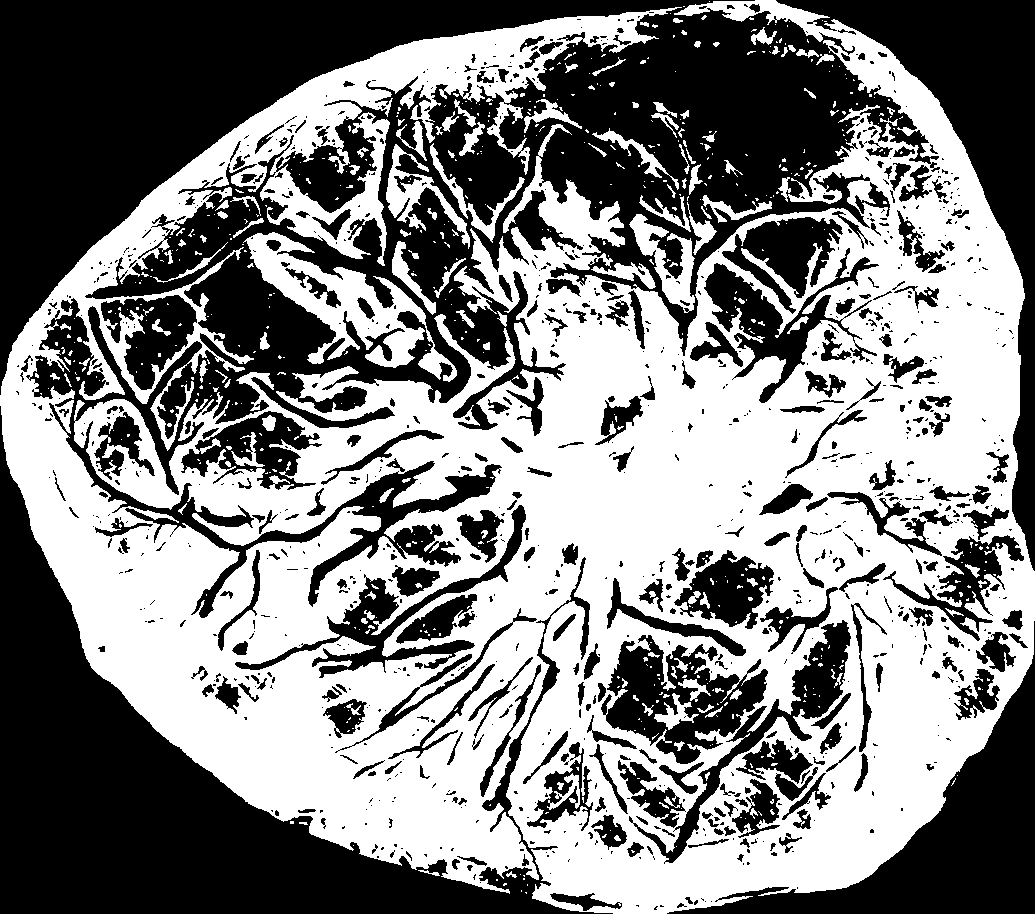
\includegraphics[width=0.8\textwidth]{shitty_threshold}
%			\caption{Luminance/brightness thresholding is bad.}
%			% this should go early in your talk, showing that the problem is kind of frustrating and visually solvable  ish.
%			\label{fig:color-thresholding-sucks}
%		\end{figure}
		
	
	\section{Research Goals}
	Our present work is to improve upon the vascular network extraction
	developed in \cite{huynh2013filter} and test our extraction against the manual traces developed.